% !TeX TXS-program:bibliography = txs:///biber
\documentclass[unknownkeysallowed]{beamer}
\usetheme{UniKlu}
\usepackage[backend=biber,style=apa,sorting=nty, bibencoding=utf8]{biblatex}
\addbibresource{refs.bib}


\usepackage{xcolor}
\usepackage{wrapfig}

\title{Collective Self-awareness in Multi-Robot Systems}
\author{Mohammad Rahmani}
\institute{DECIDE Doctoral School}

\begin{document}
\begin{frame}
	\maketitle
\end{frame}

\begin{frame}{Biological Self-awareness (SA)}
	\begin{wrapfigure}{r}{0.6\textwidth}
		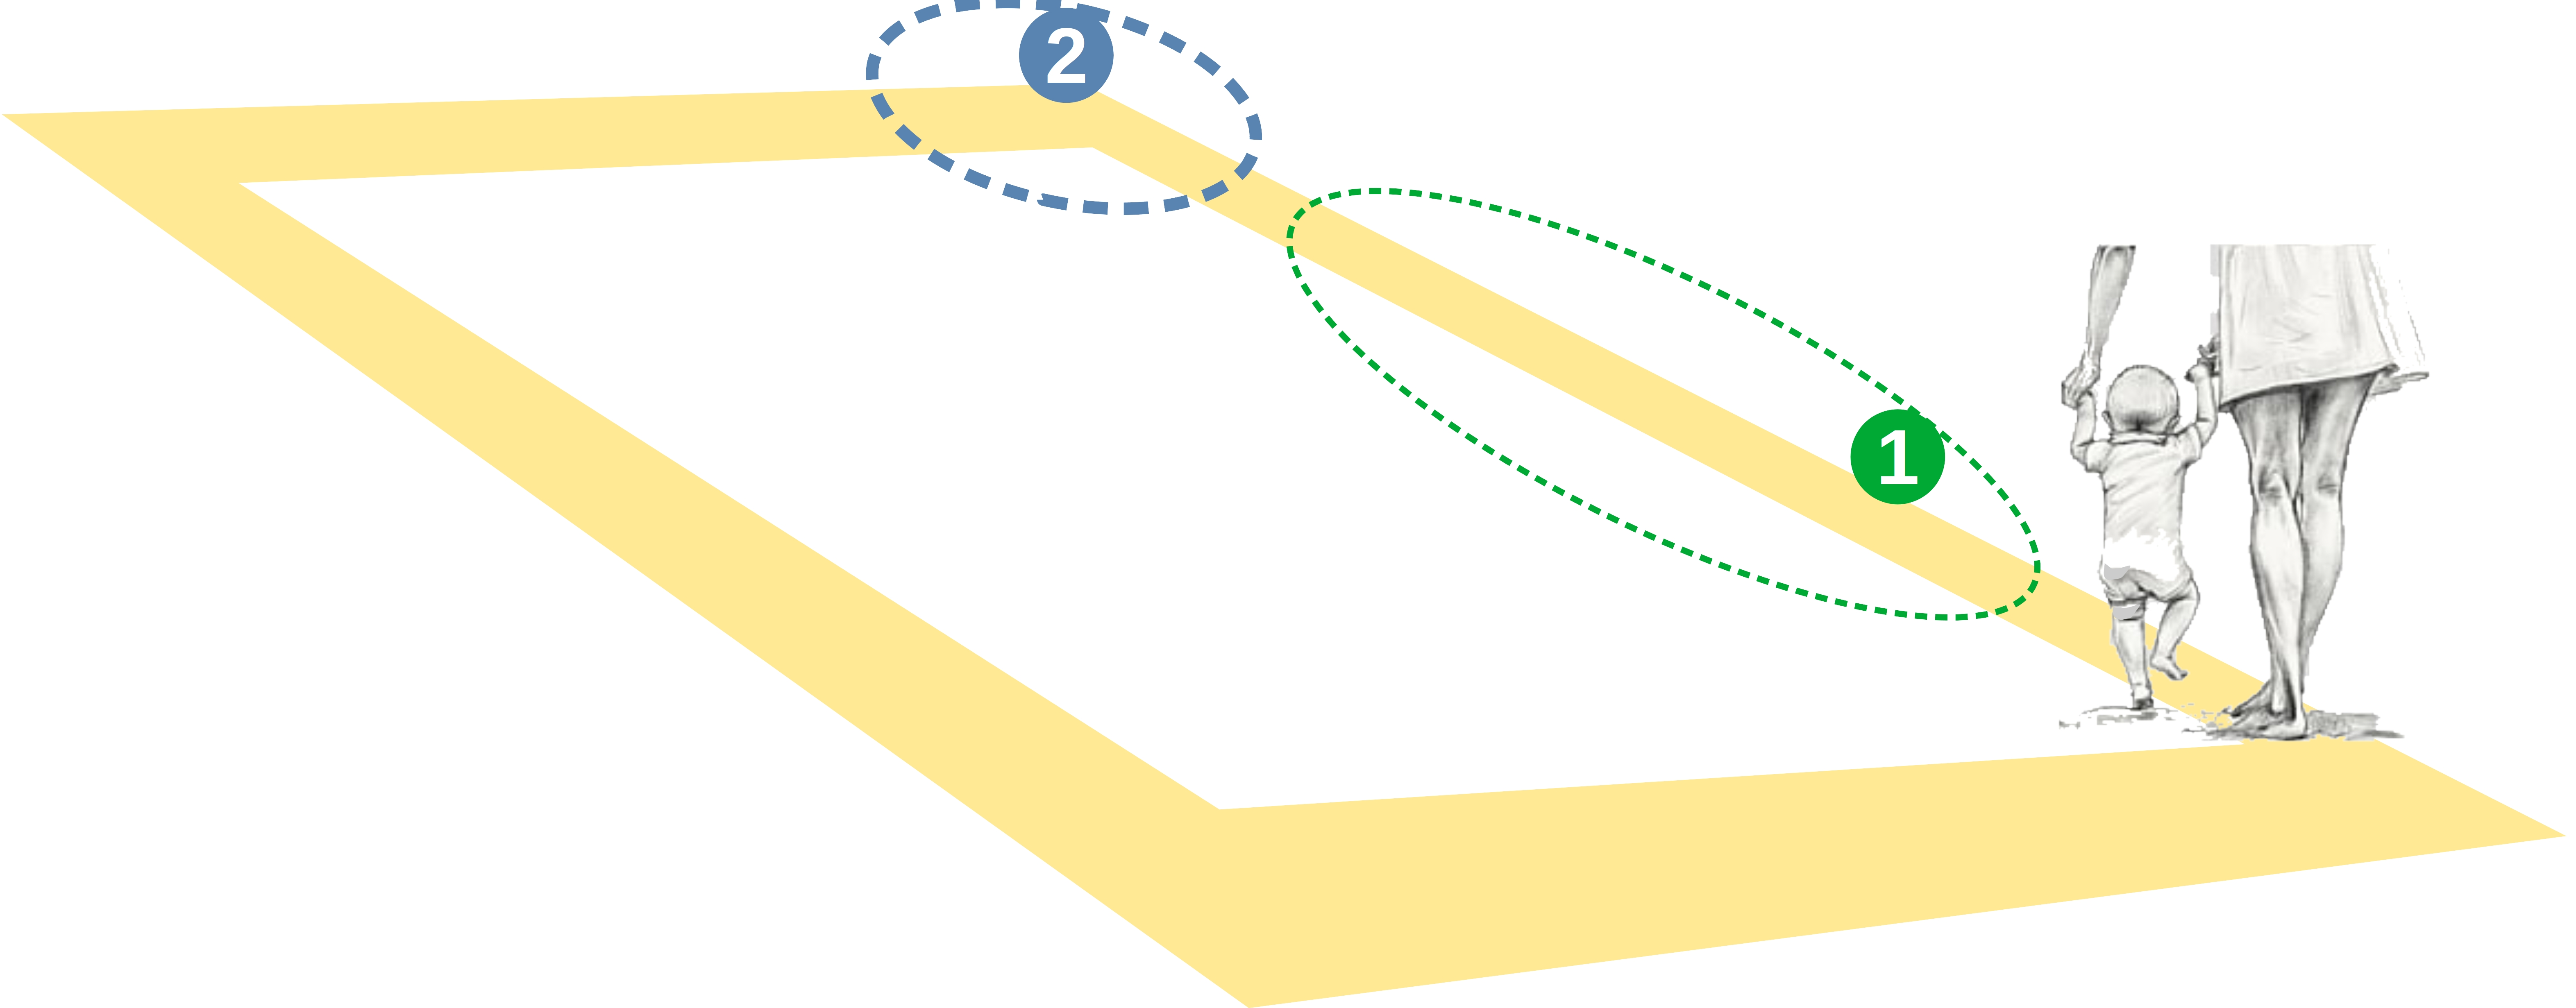
\includegraphics[width=1\linewidth]{/home/donkarlo/Dropbox/projs/research/artificial-intelligence/self-awareness/docs/assets/mother-baby.jpg} 
	\end{wrapfigure}
	A baby walking around a rectangular courtyard for the \textbf{first time} with her mother.
	\begin{itemize}
		\item Gradually she learns how to use her feet when moving \textbf{straight} and moving on \textbf{corners}
	\end{itemize}
\end{frame}

\begin{frame}{Biological SA}
	\begin{wrapfigure}{r}{0.5\textwidth}
		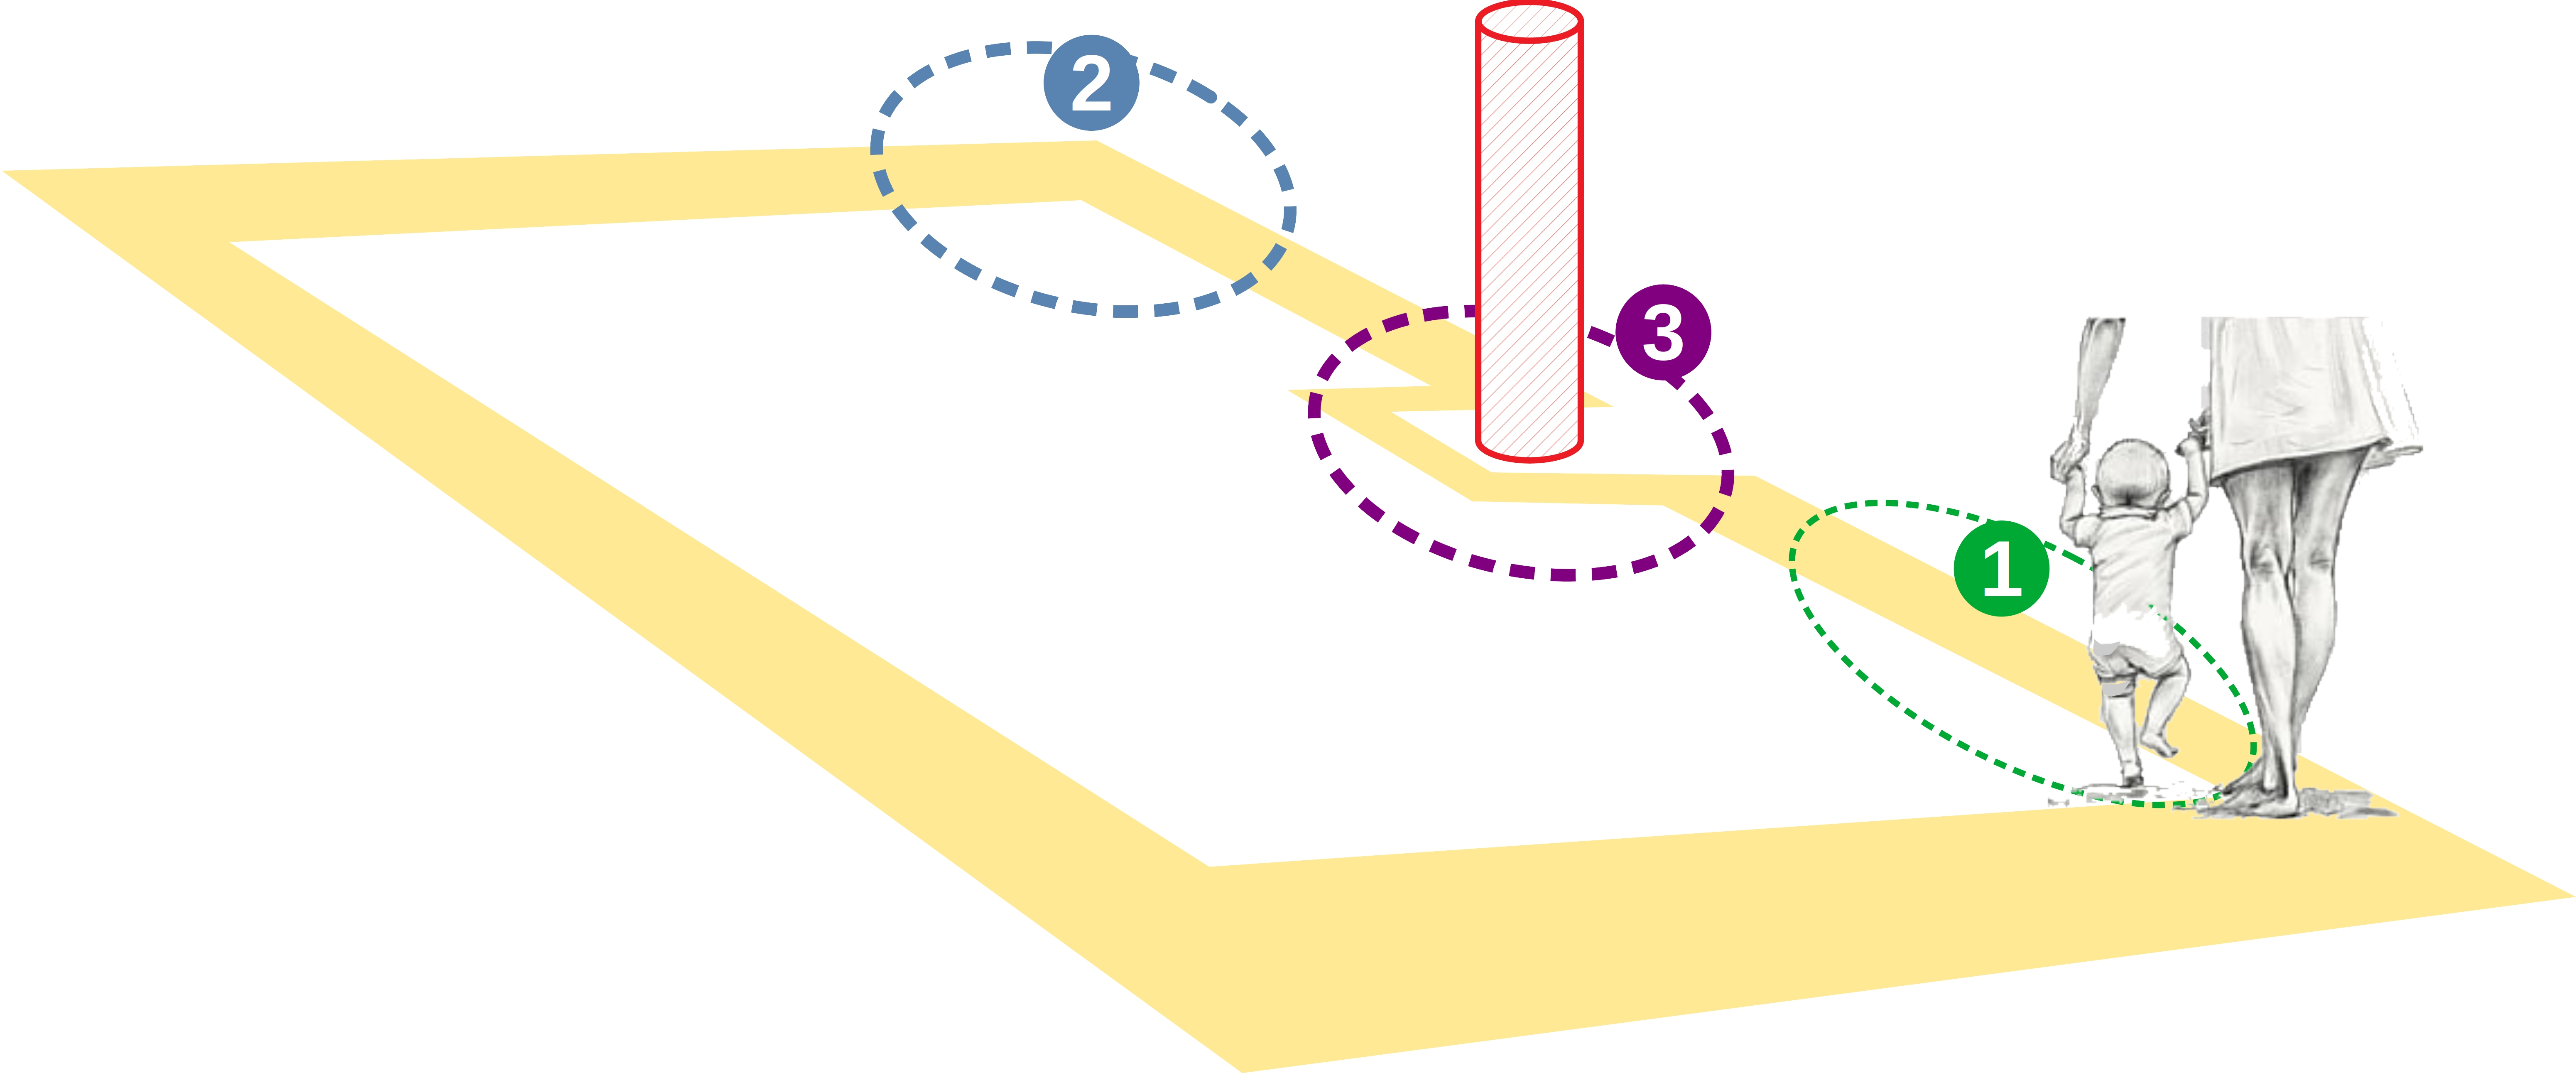
\includegraphics[width=1\linewidth]{/home/donkarlo/Dropbox/projs/research/artificial-intelligence/self-awareness/docs/assets/mother-baby-third-exp.jpg} 
	\end{wrapfigure}
	The next time, when the path is interrupted by a column, the baby learns how to use its feet to \textbf{turn around an obstacle} with the help of her \textbf{mother}. Now the baby can
	\begin{itemize}
		\item distinguish a \textbf{new} experience from the previous \textbf{(Self-awareness)}
		\item \textbf{memorize} it to predict its future 
		\item \textbf{invoke} it when necessary
		\item relate \textbf{vision} with \textbf{feet} to repeat the right experience \textbf{without} \textbf{mother}
	\end{itemize} 
\end{frame}

\begin{frame}{Single Intelligent Agents (IA) SA}
	\begin{wrapfigure}{r}{0.5\textwidth}
		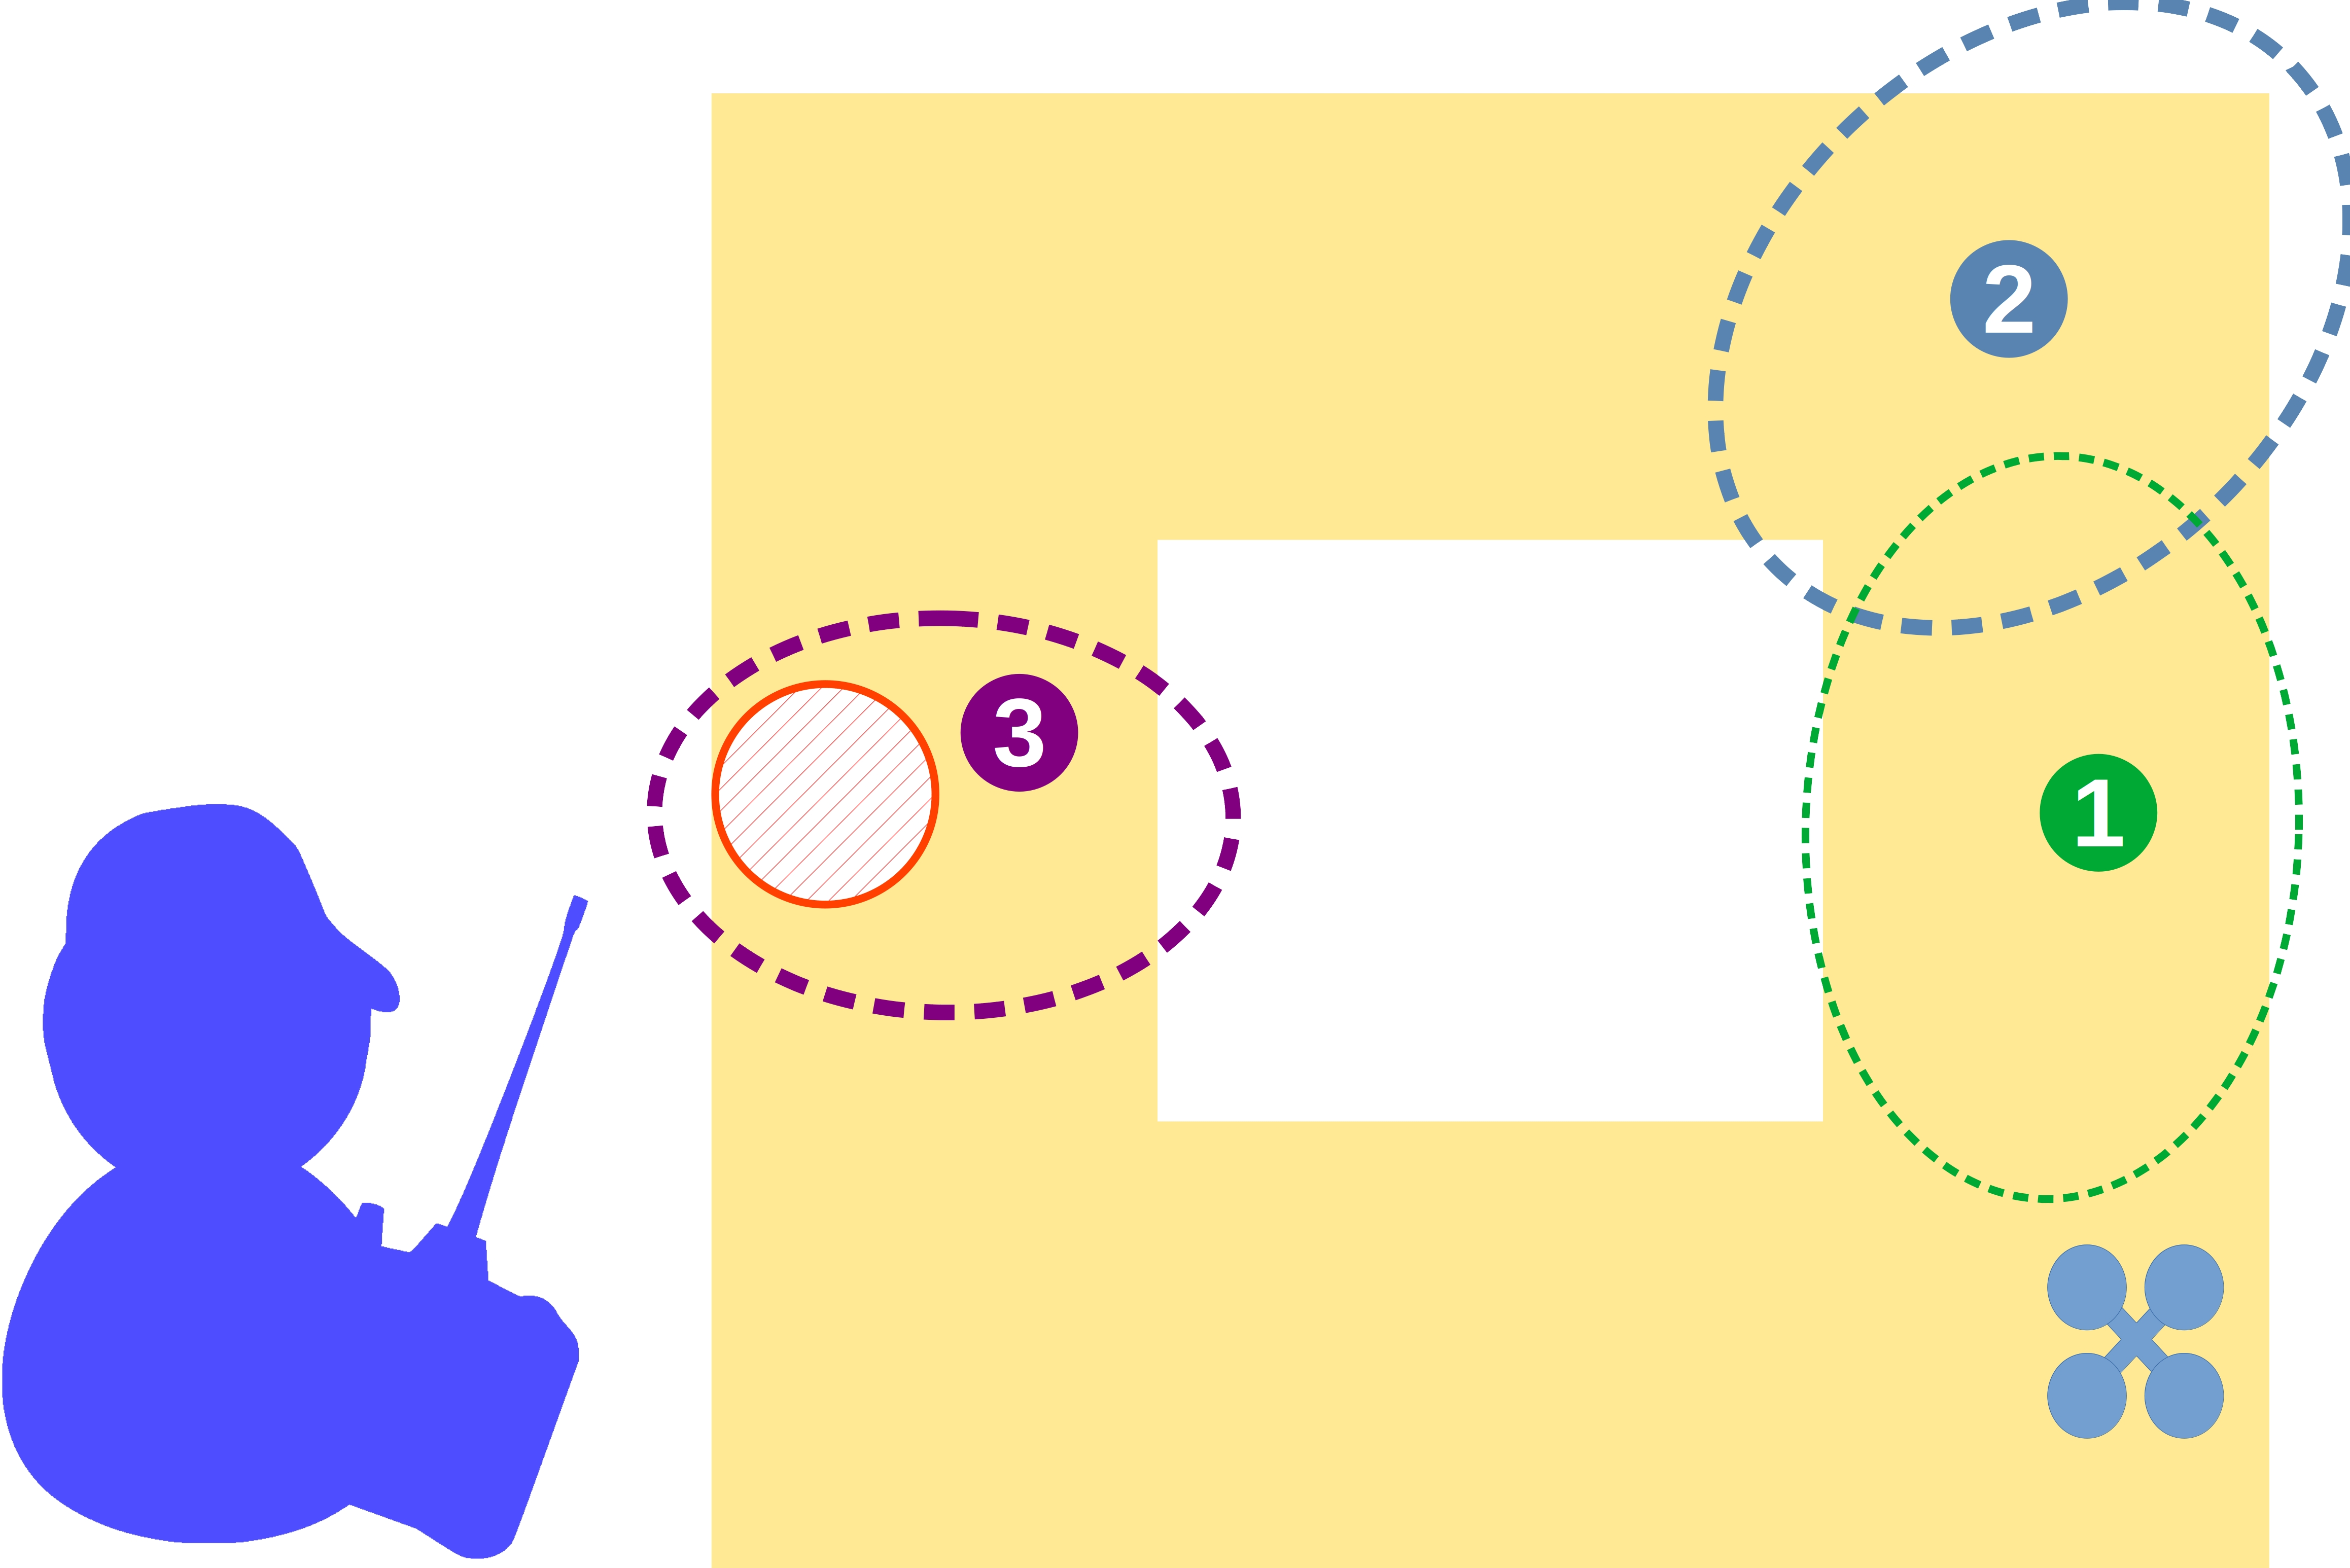
\includegraphics[width=1\linewidth]{/home/donkarlo/Dropbox/projs/research/artificial-intelligence/self-awareness/docs/assets/pilot-drone.jpg} 
	\end{wrapfigure}
	A \textbf{human pilot} flies a drone. Similar to biological SA, an IA should be able to 
	\begin{itemize}
		\item \textbf{encode sub-experiences} such as \textbf{straight/corner movement} 
		\item \textbf{distinguish} news experiences \textbf{(collision avoidance)} 
		\item \textbf{invoke} them when \textbf{necessary}
		\item \textbf{Relate} its rotors' power to its \textbf{camera} to repeat the right experience without \textbf{pilot}
	\end{itemize} 
\end{frame}

\begin{frame}{Collective Intelligent Agents (IA) SA}
	\begin{wrapfigure}{t}{0.5\textwidth}
		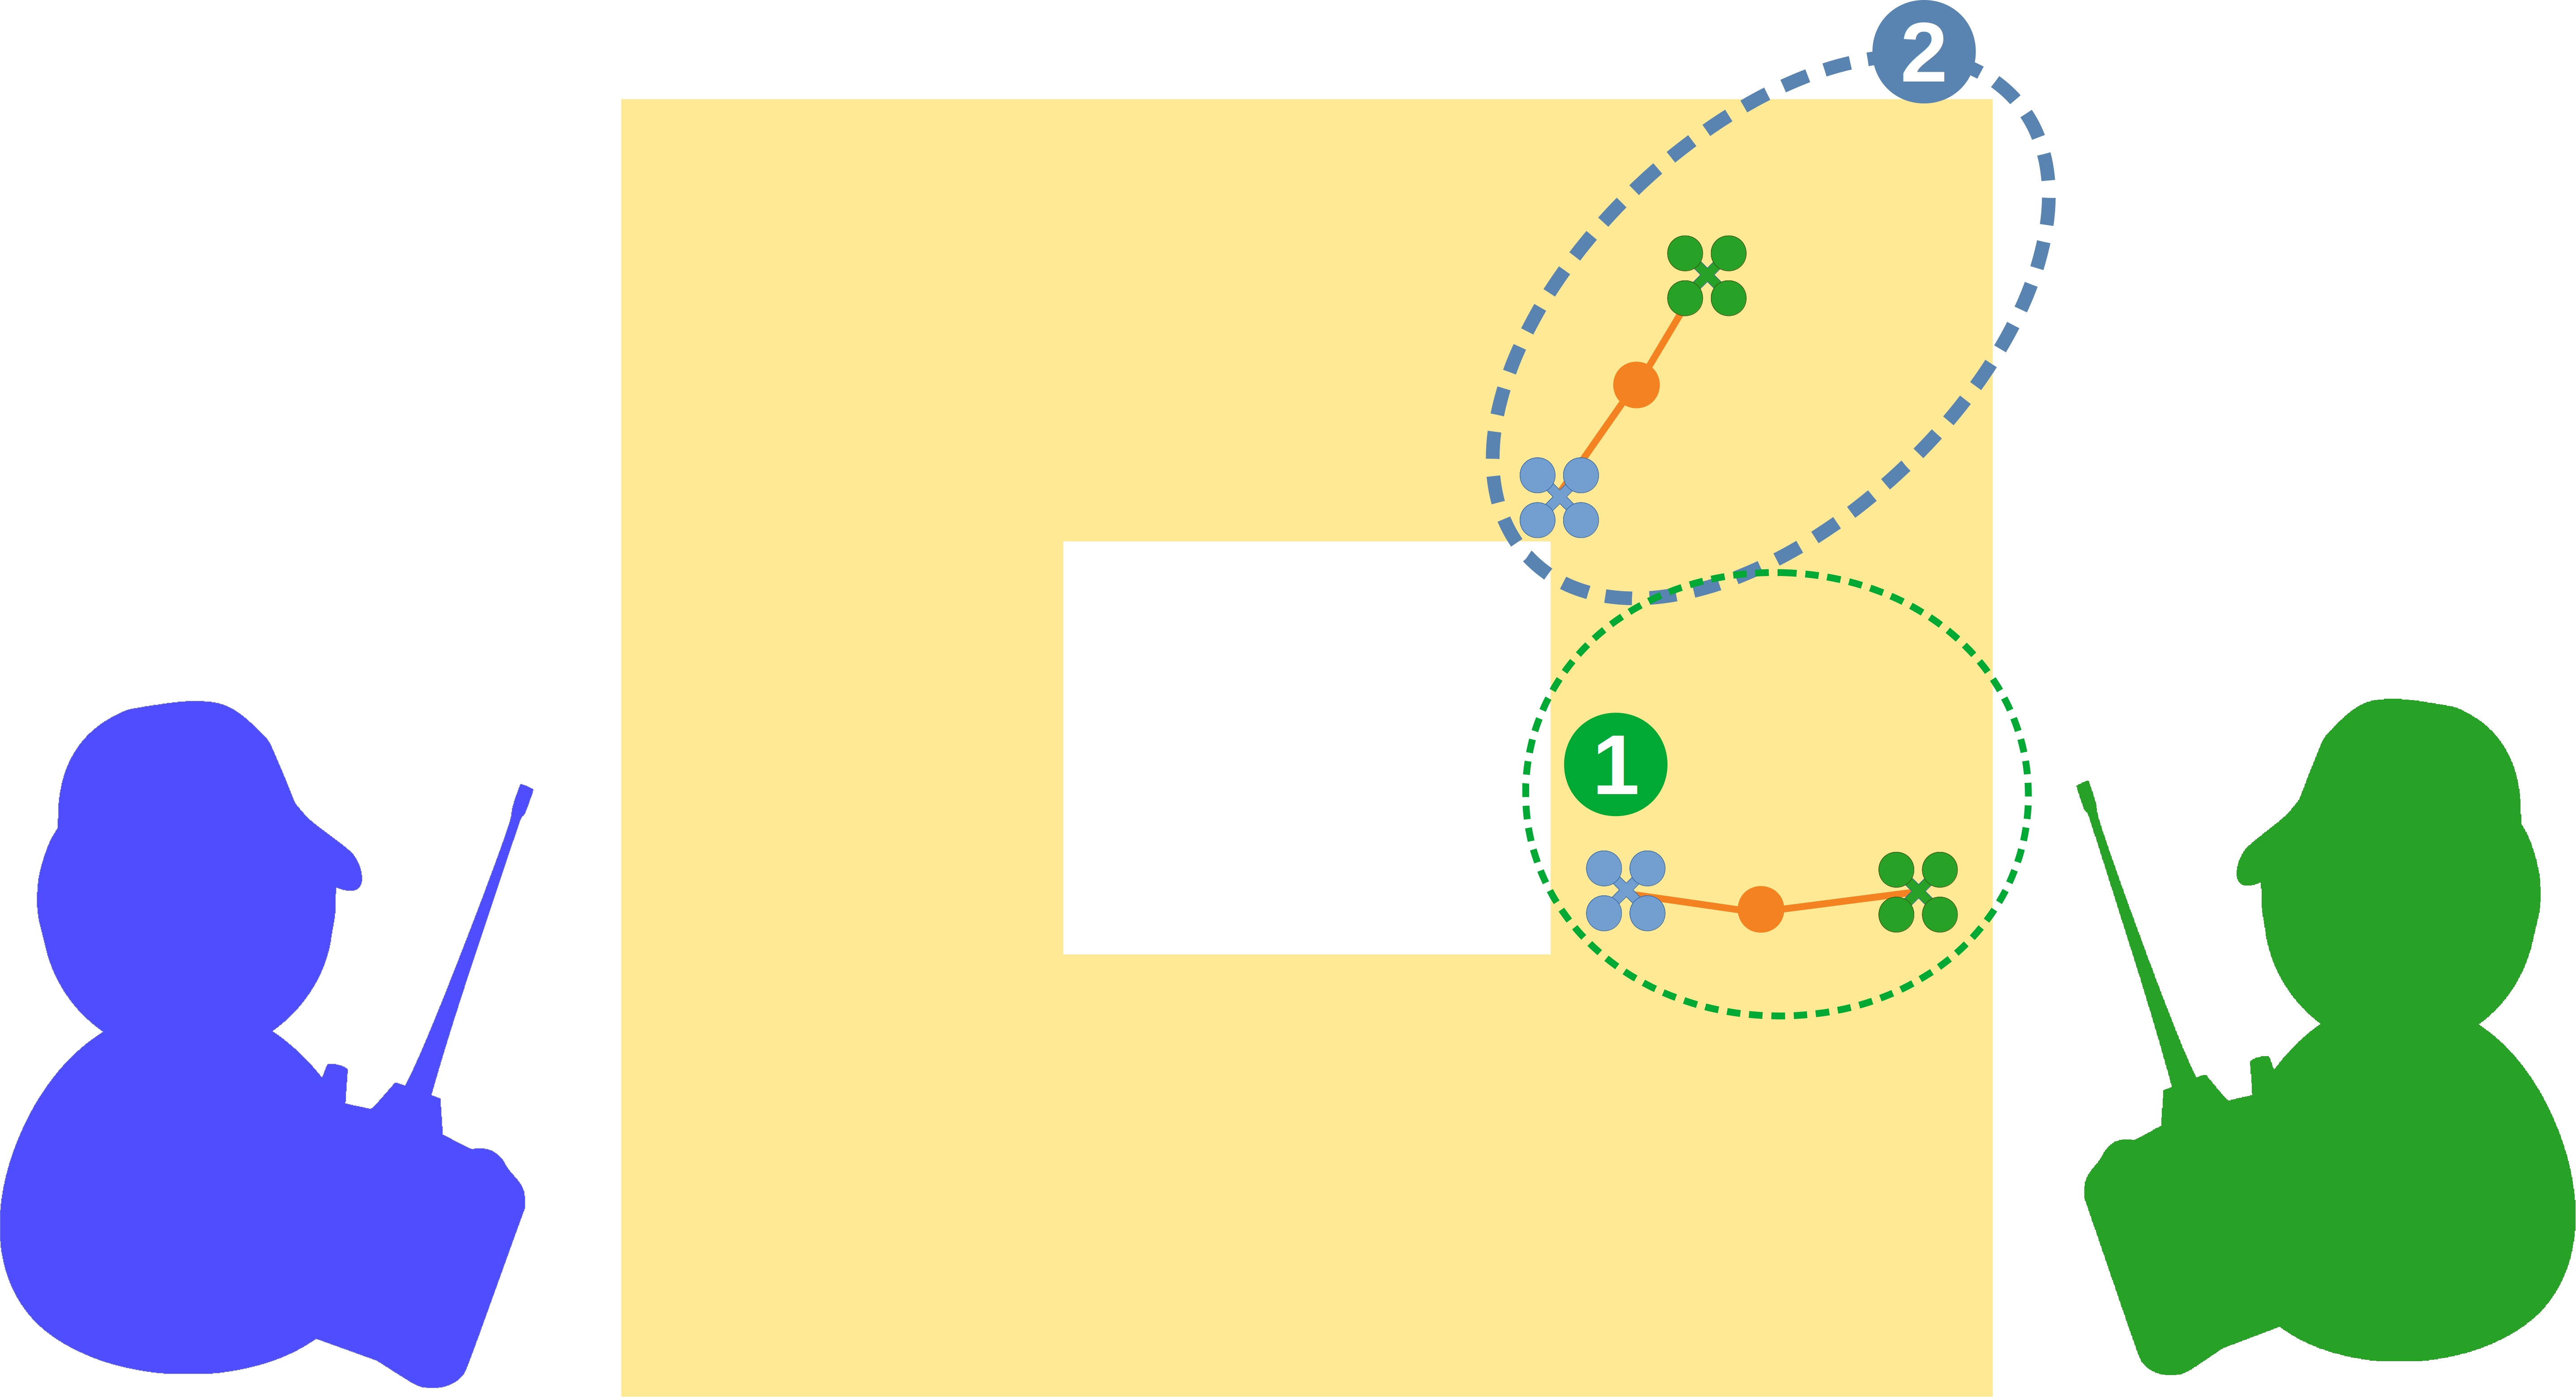
\includegraphics[width=1\linewidth]{/home/donkarlo/Dropbox/projs/research/artificial-intelligence/self-awareness/docs/assets/pilot-drone-collective-initial.jpg} 
	\end{wrapfigure}
	In single awareness we were after making a single IA aware of experiences such as moving \textbf{straight}, \textbf{turning} and \textbf{collision avoidance}. In \textbf{collective} awareness we are after \textbf{distinguishing} experiences such as 
	\begin{itemize}
		\item \textbf{Moving along} \textbf{each} other
		\item \textbf{Turning around} \textbf{each} other
	\end{itemize}
\end{frame}

\begin{frame}{Collective Intelligent Agents (IA) SA - New experience}
	\begin{wrapfigure}{t}{0.5\textwidth}
		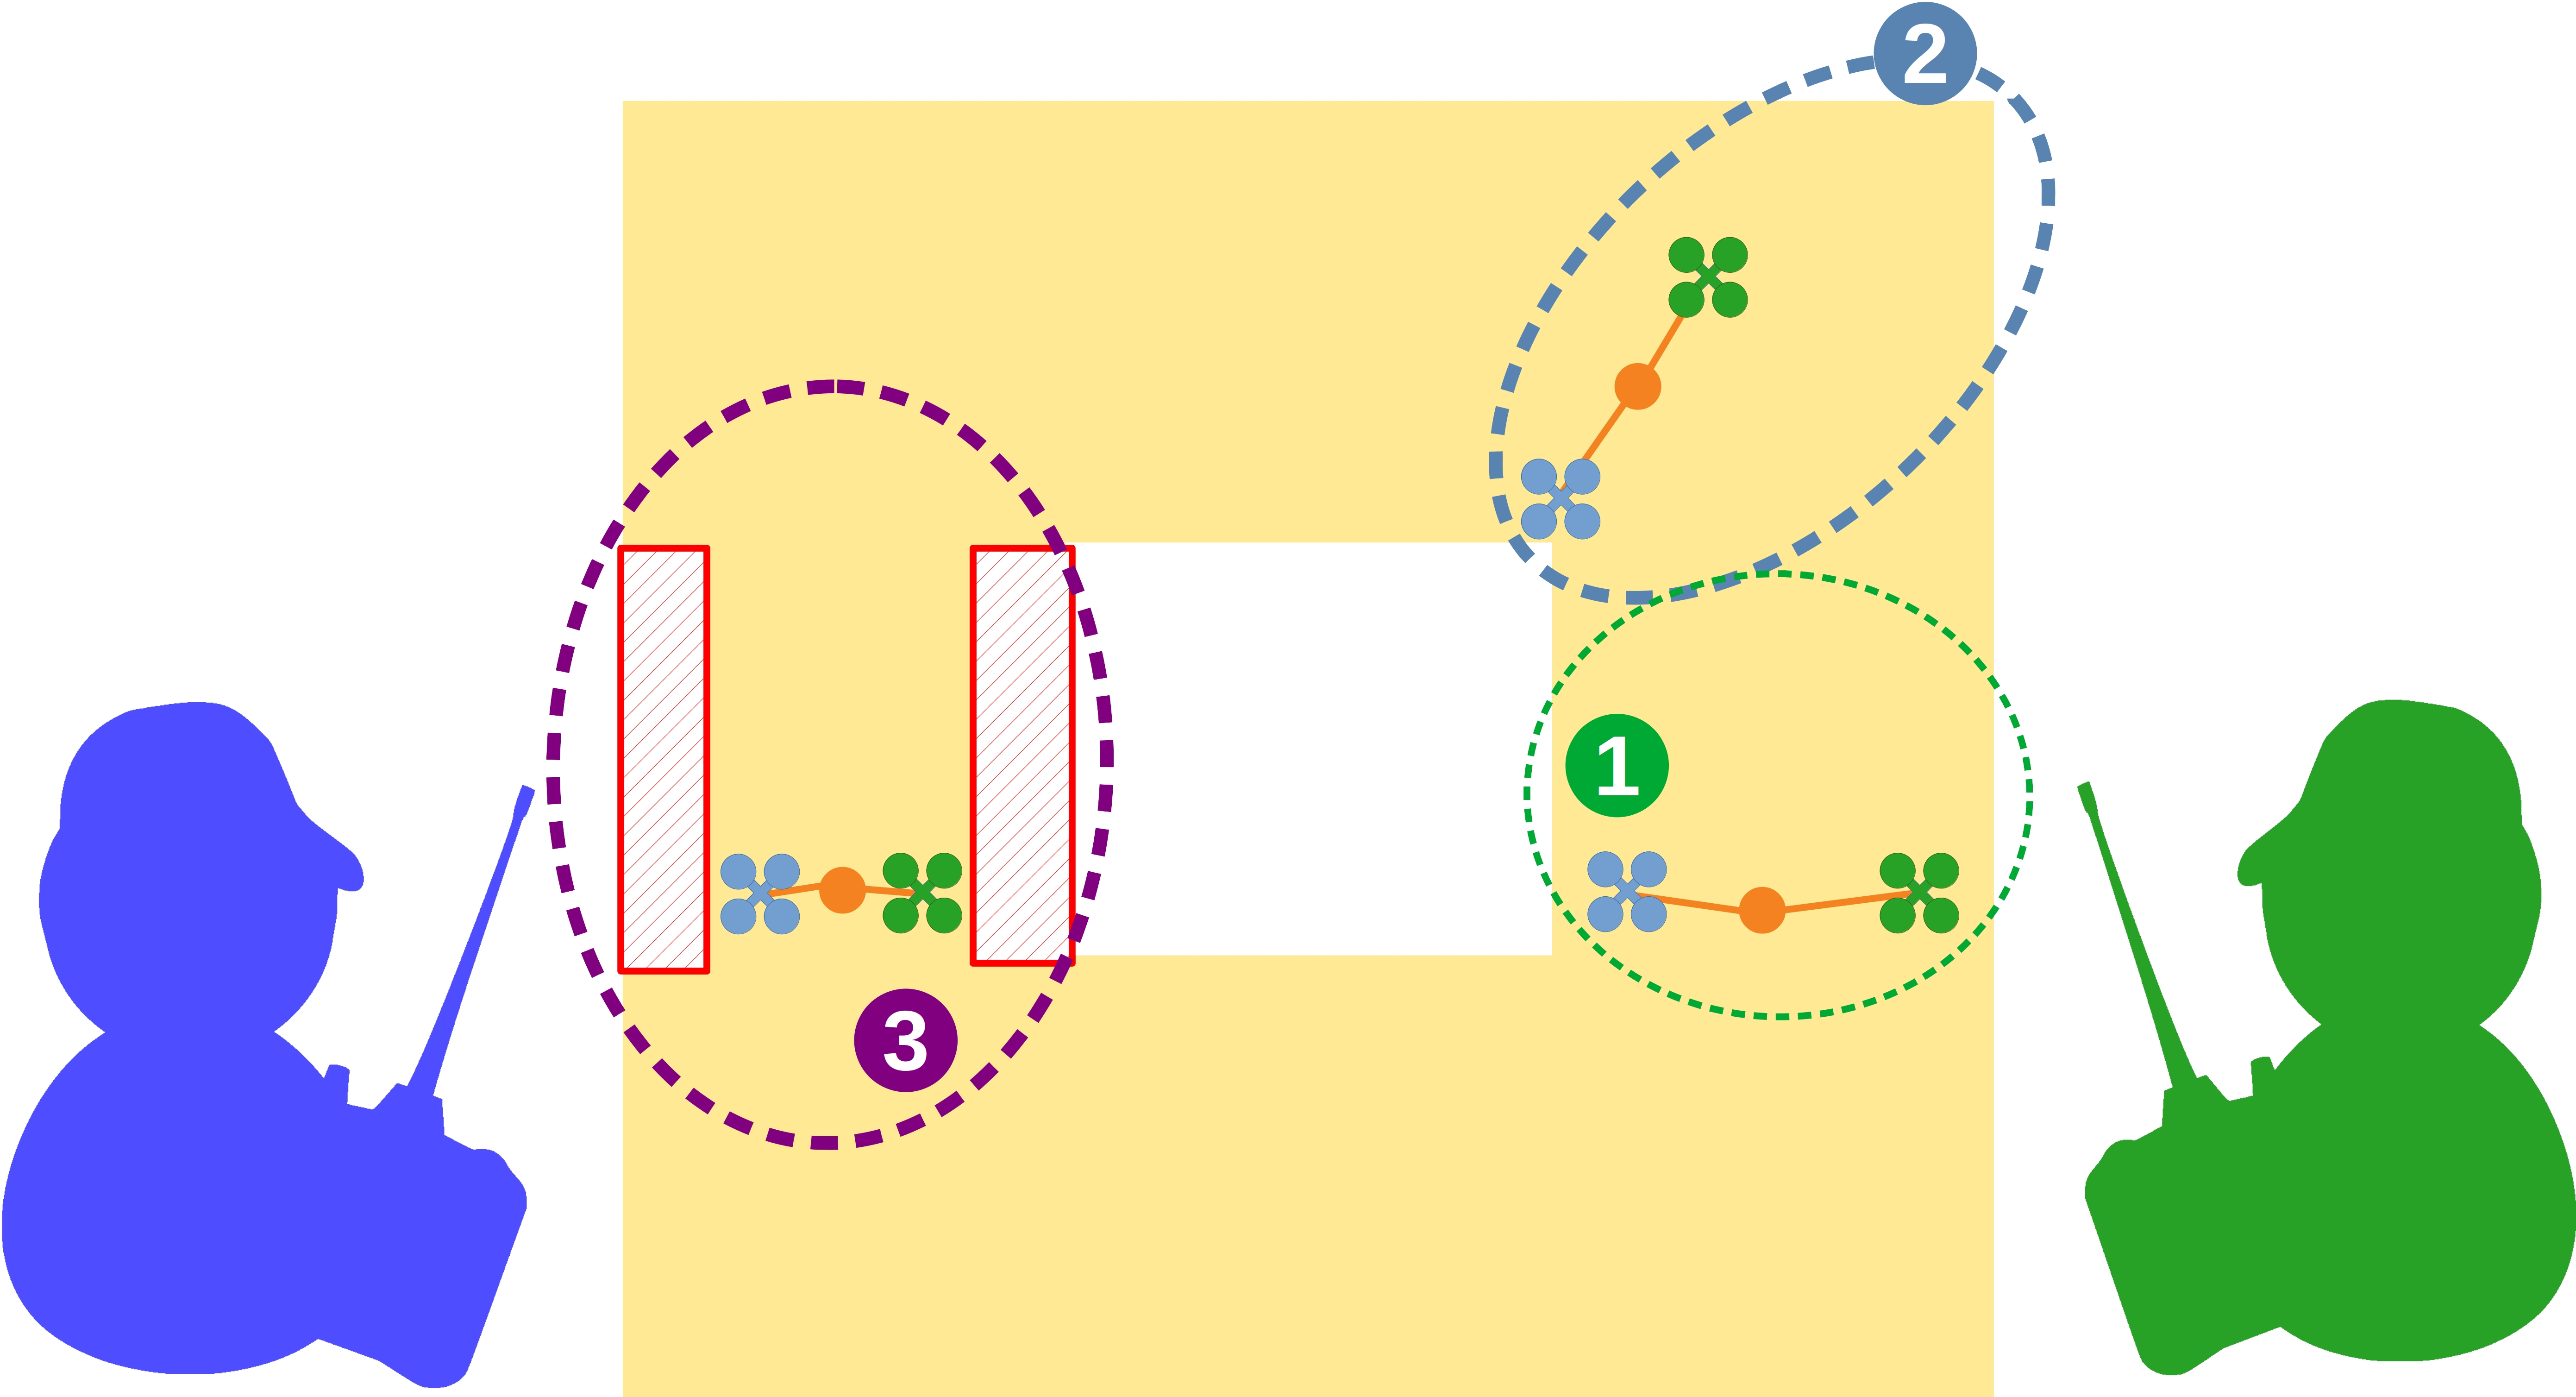
\includegraphics[width=1\linewidth]{/home/donkarlo/Dropbox/projs/research/artificial-intelligence/self-awareness/docs/assets/pilot-drone-collective.jpg} 
	\end{wrapfigure}
	If in a new experiment, the two pilots face a narrow corridor, then the two drones should be able to memorize the solution as:
	\begin{itemize}
		\item \textbf{Getting closer} to \textbf{each} other
		\item Invoke it without pilots then after
	\end{itemize}
\end{frame}

\begin{frame}{Summary}
	Not much studies have been done in Collective awareness. The \textbf{Goals} of our research are as follows according to the given example: If two drones are piloted by two \textbf{human} pilots,
	\begin{itemize}
		\item We want them to encode an initial experience in their memory. Like turning around a square. 
		\item We want them to be able to break the experience into smaller pieces such as \textbf{moving along each other} or \textbf{turning around each other} for 90 degrees to have better \textbf{prediction} of their future state given such \textbf{abstract behavioral states}
	\end{itemize}
\end{frame}

\begin{frame}{Summary - 2}
	\begin{itemize}
		\item If in a new experience, an \textbf{abnormal} case happens (\textbf{prediction doesn't match observation}) for which the \textbf{intervention} of human pilots is needed (eg: arriving to a narrow corridor where they should fly closer to each other), then they should be capable of \textbf{distinguishing} it for memorization. 
		\item They should be able to memorize the new experience as a\textbf{ new version} of previous experience. 
		\item They should be able to \textbf{invoke} appropriate experiences according to their observations for \textbf{current state estimation} and \textbf{future state prediction} without the pilots
	\end{itemize}
\end{frame}

\end{document}
